% BREDEX LaTeX Template
%  \documentclass is either ``bxreport'' or ``bxarticle''
%                 option is bxpaper
%% \documentclass{bxarticle}
%% % ----------------------------------------------------------------------
%% \begin{document}
%% \title{}
%% \author{}
%% % \author*{Hauptautor}{Liste der Nebenautoren}
%% \maketitle
%% % ----------------------------------------------------------------------
%% \bxversion{0.1}
%% %\bxdocinfo{STATUS}{freigegeben durch}{freigegeben am}{Verteilerliste}
%% \bxdocinfo{DRAFT}{}{}{}
%% % ----------------------------------------------------------------------

%% \end{document}
\index{Preferences!Object Mapping}
\index{Object Mapping!Preferences}

\begin{figure}[h]
\begin{center}
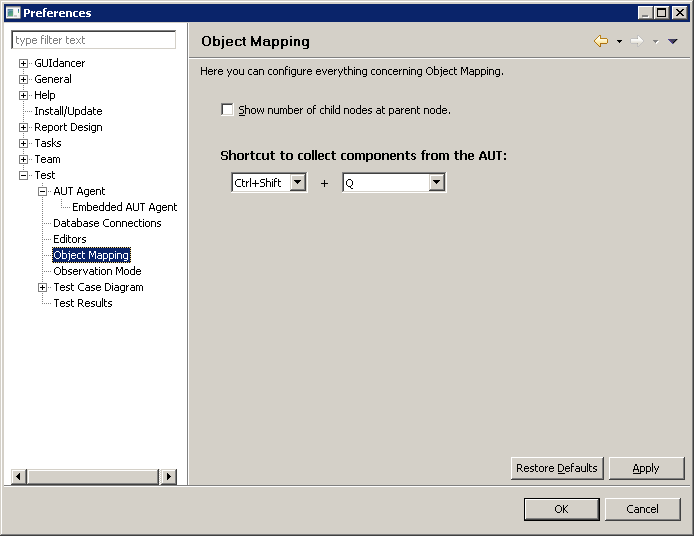
\includegraphics[width=0.6\textwidth]{Tasks/Preferences/PS/objectmappingprefs}
\caption{Object Mapping Preference Dialog}
\label{objectmappingprefs}
\end{center}
\end{figure}

You can access the object mapping preferences from \bxname{Test - Object Mapping} in the preferences dialog. 
\begin{enumerate}
\item Select whether you want \app{} to display how many nodes are contained in each category in the \gdomeditor{}. 
\item Choose which keystrokes or mouse buttons you want to use to collect components in the \gdomm{}.  
\end{enumerate}

\bxtipp{If your \gdaut{} does not accept keystrokes, set the object collection preference to a mouse button combined with a modifier key.}
